%% Template for MLP Coursework 1 / 16 October 2017 

%% Based on  LaTeX template for ICML 2017 - example_paper.tex at 
%%  https://2017.icml.cc/Conferences/2017/StyleAuthorInstructions

\documentclass{article}

\usepackage[T1]{fontenc}
\usepackage{amssymb,amsmath}
\usepackage{txfonts}
\usepackage{microtype}
\usepackage{enumitem}
\usepackage{float}

% For figures
\usepackage{graphicx}
\usepackage{subfigure} 

% For citations
\usepackage{natbib}

% For algorithms
\usepackage{algorithm}
\usepackage{algorithmic}

% the hyperref package is used to produce hyperlinks in the
% resulting PDF.  If this breaks your system, please commend out the
% following usepackage line and replace \usepackage{mlp2017} with
% \usepackage[nohyperref]{mlp2017} below.
\usepackage{hyperref}
\usepackage{url}
\urlstyle{same}

% Packages hyperref and algorithmic misbehave sometimes.  We can fix
% this with the following command.
\newcommand{\theHalgorithm}{\arabic{algorithm}}


% Set up MLP coursework style (based on ICML style)
\usepackage{mlp2017}
\mlptitlerunning{MLP Coursework 4 (\studentNumber)}
\bibliographystyle{icml2017}

\DeclareMathOperator{\softmax}{softmax}
\DeclareMathOperator{\sigmoid}{sigmoid}
\DeclareMathOperator{\sgn}{sgn}
\DeclareMathOperator{\relu}{relu}
\DeclareMathOperator{\lrelu}{lrelu}
\DeclareMathOperator{\elu}{elu}
\DeclareMathOperator{\selu}{selu}
\DeclareMathOperator{\maxout}{maxout}

%% You probably do not need to change anything above this comment

%% REPLACE this with your student number
\def\studentNumber{s1700260, s1457374, s1784849}

\begin{document} 

\twocolumn[
\mlptitle{MLP Coursework 4: Project Final Report \\
Transfer learning and dataset size\\
Group G74
}

\centerline{\studentNumber}

\vskip 7mm
]

\begin{abstract} 
Write This Last.
\end{abstract} 

\section{Introduction}
\label{sec:intro}

Large-scale neural networks have become increasingly prevalent in artificial intelligence [INSERT REFERENCE HERE]. Such architectures effectively solve computer vision problems that were previously considered difficult to address using traditional symbolic manipulation [INSERT REFERENCE HERE]. One concern with modern neural networks is that their performance scales with the quantity of data used to train them, as demonstrated in our previous piece of research [INSERT REFERENCE HERE]. This concern is a problem for individuals or institutions with small amounts of data that want to implement these architectures as solutions, or for research purposes.

Data driven techniques exist, such as data augmentation [INSERT REFERENCE HERE], which help solve this problem [footnote: see our previous paper for a further explanation]. However, to draw from our previous research [INSERT REFERENCE HERE] we investigate alternative, machine learning based approaches, specifically transfer learning [INSERT REFERENCE HERE] as a method to improve the performance of neural network architectures that utilise small amounts of data. These techniques allow us to use the knowledge that a given (pre-trained) network already has and adapt the architecture to suit our requirements [INSERT REFERENCE HERE].

The objective of transfer learning is to use the knowledge acquired by an existing network that was built to solve a similar task and improve the generalization. The main idea is to try to adapt that previous knowledge to the new problem to be solved. One of the advantages of this technique is that the solution for the new problem does not have to start from scratch. Prior work can be re-utilised which is important when the resources are limited. This situation is specially true for convolutional neural networks which, depending on the size of the architecture, can require an important amount of computational power.

There exist a number of pre-trained neural networks to solve classification tasks in the field of computer vision. One of them is the Visual Geometry Group network (VGG net)[INSERT REFERENCE HERE]. This network implements a simple yet deep architecture with several convolutional layers. There are several configurations that vary the number of convolutional layers among 11, 13, 16, and 19. In every configuration the architecture includes maximum pooling layers of dimensions 2x2 and stride 1. The convolutions are performed using 3x3 filters with stride and pad of 1. Finally, ReLU activations after each convolution are utilised.

VGG net was firs used in the ImageNet Challenge 2014[INSERT REFERENCE HERE], which means that is was originally trained using the Imagenet dataset [INSERT REFERENCE HERE]. However, the network has also been trained in other datasets like CIFAR-10 [INSERT REFERENCE HERE] and CIFAR-100[INSERT REFERENCE HERE]. It is important to make this distinction since each dataset has been developed for a different purpose, therefore, they have specific characteristics. The knowledge learnt from a network depends on the dataset used to train it. Thus, it is critical to know the characteristics of the dataset utilised to train the network since it will play and important role when implementing transfer learning.

ImageNet is a large-scale hierarchical image database [INSERT REFERENCE HERE]. The structure of this dataset contains 12 main groups or sub-trees. Each sub-tree contains a variable number of categories. The total number of categories is 5247, each one containing on average 600 images; thus, the total number of images in the dataset is 3.2 million. As described, ImageNet is a large and diverse dataset. However, the original version of VGG net was trained on a subset of Imagenet that contains only 1000 categories using 1.3 million images for training, 50K images for validation and 100K images for testing.



\subsection{Interim Report Findings}
\label{sec:findings}

The research questions offered within this report have been drawn from our initial findings, as documented in the interim report [INSERT REFERENCE HERE]. To aid in orientating the reader, we provide a summary of these findings here.

It was possible to demonstrate how the amount of available data impacts the performance of a convolutional neural network. Such impact was observed in the validation stage by analysing the accuracy and error of the network. In the first case, it was evident the reduction of the accuracy as the size of the dataset was reduced. In the second case, the size of the dataset directly affected the error; the smaller the dataset, the bigger the error. In both cases, the ultimate effect of such behaviour was the difficulty of the network to generalize when the amount of data is small.

Futhermore, the usage of two different but comparable databases provided some extra insights about the behaviour of the neural network. In this case the observed accuracies in the validation stage were different for each dataset in every size used to train the network. Under these circumstances, it was clear that the dataset that allowed a higher accuracy (clothes) was less challenging for the network. This means, that the features extracted by the network were more useful and relevant for one of the datasets. In the other hand, the features learned by the network did not provide enough information to reach better results for the second dataset (expressions).

Finally, we demonstrated that a simple data driven technique like data augmentation effectively improves the performance of a simple convolutional neural network. However, the benefits of this method have a limit above which no further improvement can be done. All of these findings provided the foundations and motivation for our investigation.

\section{Objectives and Research Questions}
\label{sec:obj_questions}

\subsection{Objectives}
\label{sec:objectives}

There are two fundamental objectives. The first one concerns with improving the performance of the image classification task using transfer learning under conditions of small data. The second objective investigates the effects of transfer learning on two distinct but comparable datasets. 

Furthermore, we intend to propose and utilise a framework for measuring the similarity between datasets using a modified siamese neural network [INSERT REFERENCE HERE] architecture.

\subsection{Research Questions}
\label{sec:questions}
Following from the conclusions drawn from our interim report, our research questions are listed below.

\begin{enumerate}
  \item How much the performance for a given classification task can be improved by using transfer learning?  
  \item How much the application of transfer learning affect two distinct but comparable datasets?
\end{enumerate}

[INSERT RESEARCH QUESTIONS ABOUT ONE SHOT LEARNING]

\subsection{Hypotheses}
\label{sec:hypotheses}
\begin{enumerate}[label=\textbf{H.\arabic*}]
  \item \label{h:1} Transfer learning will provide a performance benefit with respect to the generalisability (measured through validation accuracy) for the given classification task in conditions of small data.
  \item \label{h:2} Transfer learning will provide a larger performance boost when the size of the dataset used to initially train the model is small rather than large.
 \end{enumerate}

Within the remainder of this report a section that outlines the methodologies utilised to conduct our research [INSERT SECTION REFERENCE] is initially given. Thereafter, all experimental results are presented [INSERT SECTION REFERENCE] and a review of related work is provided [INSERT SECTION REFERENCE]. Finally, a set of conclusions are drawn [INSERT SECTION REFERENCE].

\section{Methodology}
\label{sec:methodology}

\subsection{Simple Transfer Learning}
\label{sec:transferlearninng}

\subsubsection{\textbf{Chosen Model}}

We decided to select the VGG net configuration with 16 convolutional layers (hereinafter referred as VGG16) to transfer its knowledge into the clothes and expressions datasets. As previously mentioned, this network is quite simple and deep, thus, the expectation is that the knowledge contained in this network will be sufficient to increase the generalisability of the classification tasks using both datasets.

Since the available versions of VGG16 have been trained with different datasets, we decided to use the knowledge obtained from ImageNet rather than other options like CIFAR-100. The main reason for this decision is the number of classes from the subset of ImageNet to train the network (1000) which is much bigger than the number of classes from CIFAR-100 (100). The expectation is that the knowledge from ImageNet is wider, therefore, it can provide better results when transferring that knowledge into new datasets.


\subsubsection{\textbf{Configuration}}
The configuration to adapt the knowledge from VGG16 into the current task is made of two stages. The first one consists of extracting part of the knowledge from VGG16. One of the main interests is to extract a sufficient number of relevant features to increase the generalization for the classification task. This situation can be accomplished by using the knowledge from the convolutional layers. The second part consists in the adaptation of the extracted knowledge. This goal is accomplished by discarding the original fully connected layers of VGG16. Then, a new set of fully connected layers adapted for the current task are implemented. Thus, the configuration is made of the convolutional layers from VGG16 connected to custom fully connected layers adapted for the current classification task.

The described configuration has a bottleneck between the convolutional layers and the fully connected ones. This bottleneck is caused by the number of convolutions that has to be done in every layer which requires a considerable amount of computational power. To reduce the impact of the described bottleneck, the transfer learning is divide into two phases.

In the first phase, only the convolutional layers are utilised. The knowledge obtained from these layers is not modified. That means that their parameters from those layers are not updated while using the clothes and expressions datasets. Under these circumstances, the images from the datasets are passed through the convolutional layers, and the output from the last one is stored for the second phase.

This process can be seen as a feature extraction stage. The raw images are converted from their original representation to a new one. The original representation of the images provides information about the pixel intensity. After passing the images through the convolutional layers, the pixel intensity information is converted to other of type of information based on the local spatial correlation of the pixels which is obtained with the convolutions.

The process of converting the images from their original representation to another using convolutional layers is computational expensive. However, one of the benefits it provides is the dimensionality reduction of the representation of the images. Each input image is converted from a representation of 4096 (64x64) pixel intensities to a representation of 2048 new features. This means a reduction in the dimensionality of the images of 50\%.

After the images have been converted to a new representation through the convolutions, they are used to feed the second part of the configuration which corresponds to the fully connected layers. There are no limitations about the options that can be used in this stage. Therefore, three alternatives have been defined. The main difference among them is the number of fully connected layers.

In the first option, only one fully connected layer is defined. This option provides 205,607 trainable parameters. The second alternative adds another fully connected layer on top of the one from the first option. The total number of parameters for this alternative 210,307 parameters. For the final alternative a new fully connected layer is added on top of the previous ones. The final number of parameters for this option is 211,407.

In every set of fully connected layers, a L2 regularisation strategy is used. The main objective of this strategy is to reduce the chances of overfitting, which is especially important for small data. Each layer uses a uniform parameter initialisation strategy. This kind of initialisation allows to have the activation done in the plateau region of a sigmoid function. Non linear activation functions are added following the convolutional layers. For the output layer, a softmax activation with a categorical cross entropy error loss is implemented. The implemented learning rule is Adam.

\subsection{one shot learning/transfer learning by learning similarity}
\label{sec:oneshot}

\subsubsection{\textbf{Siamese Neural Network}}
In the previous section, transfer learning is achieved by utilizing and fine tunning weights in pre-trained large scale model which aims 
at solving machine learning task when insufficient/few data are acquired.Inspired by Koch et.al 2015 idea in using Siamese network to perform one-shot learning tasks and classify unseen images which classes of test images are only seen at test time. We are interested in using alternative transfer learning method to solve the problem of insufficient target data for training, by learning to distinguish similarity between images , from related training dataset but different from the target data. This is in essence differed from the method in previous section as training data are different from (but related to) the target data to be classified. 

In the original paper, Koch et.al first trained on a subset of Omniglot dataset(character dataset similar to MNIST) and during test time, classify rest of the subset of Omniglot datashot. Siamese network first consists of blocks of convolutional layer, Relu and max pooling layers followed by full connected layers and L1 distance layer which allows the neural network to learn generic features of images and similarity between image pairs respectively. 

In this project, we proposed an augmented version of Siamese network as suggested in original paper. Since training convolutional layers could allow the neural network to learn generic features of images, replacing the convolutional layers with VGG16, which is pre-trained in Imagenet encapsulates generic and detailed features of large amount of images. This may reinforce the Moreover, since the weights of VGG16 has been trained, we hypothesized that the no. of training data needed could be reduced. As opposed to original Siamese network which still has to be trained on large amount of related training set(30k,90k and 150k pairs of training image respectively), incorporating large scale pre-trained convolutional layers as supplement would be potent.

Our model consists of first 19 layers in VGG16 followed by flatten layer which converts all features matrix from the previous layers to a equivalent n-dimensional matrix (n,) in python. These vectors are then passed to full connected layer with sigmoid activation which outputs 4096 vectors.Next, we pass these vectors to our defined L1 distance layer which calculates the l1 distance between pairs of image input as a number. Finally, we output the probability of each pair images being in the same class based on a last fully connected layer also with sigmoid activation. Binary cross-entropy is then used as loss function. To avoid overfitting, l2 regularization with $\lambda=0.0001$. 
[[PLACEHOLDER]]

\subsubsection{\textbf{Algorithm}}

[[PLACEHOLDER]]

\section{Experiments}
\label{sec:experiments}

\subsection{Simple Transfer Learning}

\subsubsection{\textbf{Motivation}}

Transfer learning is a technique that takes advantage of previous work. The objective is to adapt that prior work to the specific circumstances of a similar new problem. As demonstrated in the previous research, the size of the dataset has a direct impact in the performance of a neural network. Therefore, the experiments of this new research are aimed to evaluate the benefits of transfer learning under the conditions of small data.

\subsubsection{\textbf{Description}}

Based on the prior findings of the existence of a correlation between the available data and the performance of a neural network, the experiments are mainly focused in the behaviour of the proposed approach for different sizes of the datasets. Even though the main focus is over small sizes of datasets, the evaluation of the proposed approach is also done over other sizes in order to get more insights about the performance of the solution. Therefore, each experiment that was conducted used the following dataset sample sizes: 100\%, 10\%, 1\%, 0.1\%.

In order to search for a practical set of system parameters, we decided to also vary the activation functions after every fully connected layers. Each experiment was initially performed using a standard sigmoid function [INSERT REFERENCE HERE]. This function was selected in order to get the benefits of a uniform initialisation strategy. However, we also ran each experiment using exponential linear units (ELU) [INSERT REFERENCE HERE]. This activation function enables another kind of non-linearities. The main advantage of ELU is its gradient which is similar to the natural gradient (smooth).

Finally, we also performed a manual sensitivity analysis by varying the learning rate values from the follow pool: 0.01, 0.001, 0.0001.

Based on the description of the components in the methodology for the transfer learning approach, we configured the experiment using three sets of fully connected layers, two different types of activation functions, four dataset subsamples and a pool of three different learning rates.

Combinations of the above result in 72 different experiments for each dataset. Due to the amount of experiments and the limited computational resources, we set a fixed number of epochs for every experiment (20), and a fixed size for the mini-batches used for the stochastic gradient descent calculation (50).

After running the aforementioned experiments, we analysed the results based on the validation accuracy. Then, we selected the configurations that get the highest values for validation accuracy for dataset sizes of 1\% and 0.1\%. For further investigation we then performed new experiments with higher number of epochs (200) to analyse the behaviour of the fully connected part of the architecture under conditions of small data.

\subsubsection{\textbf{Results}}

In order to compare the results of the current experiments to the baselines described in the previous report, the analysis of the transfer learning experiments is focused on the validation accuracy. Overall, there is still an evident reduction of the performance of the architecture related to the size of the datasets, as shown in Figure \ref{fig:tf_clot} and Figure \ref{fig:tf_exp}.

\begin{figure*}
    \vskip 5mm
        \begin{center}
            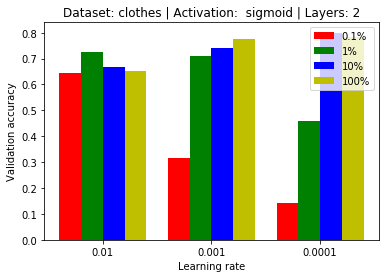
\includegraphics[scale=0.5]{accuracy_reduction_00.png}
            \caption{Validation accuracy comparison for the clothes dataset. The configuration with two fully connected layers and Sigmoid activations allows the highest accuracy for the smallest size of the dataset.}
            \label{fig:tf_clot}
        \end{center}
    \vskip -5mm
\end{figure*}

\begin{figure*}[tb]
    \vskip 5mm
        \begin{center}
            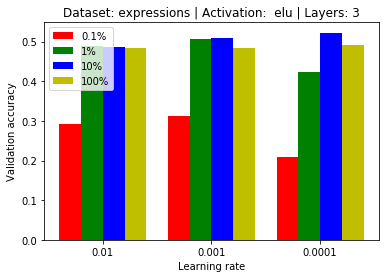
\includegraphics[scale=0.5]{accuracy_reduction_01.png}
            \caption{Validation accuracy comparison for the expression dataset. The configuration with three fully connected layers and ELU activations allows the highest accuracy for the smallest size of the dataset.}
            \label{fig:tf_exp}
        \end{center}
    \vskip -5mm
\end{figure*}

Figure \ref{fig:tf_clot} shows the effect of the learning rate for every size of the clothes dataset. It is clearly evident how differently that hyper-parameter affects the validation accuracy of the system for each size. While the learning rate reduces, the validation accuracy when the sizes are 0.1\% and 1\% increases. In the other hand, the increase of the learning rate reduces the validation accuracy when the sizes are 10\% and 100\%. This behaviour might be an indicator of the relationship between the number of available training samples and the learning rate when the batch size is kept constant.

Figure \ref{fig:tf_exp} shows the effect of the learning rate for every size of the expressions dataset. Similarly, the size of the learning rate has a positive impact for small sizes, and a negative one for bigger sizes. However, the validation accuracy is reduced for small sizes when the learning rates goes from 0.001 to 0.01 . This situation might indicate the existence of a peak where the benefits of a large learning for small sizes start to decrease.

For each dataset, the configurations that provide the highest accuracy for the smallest dataset size are quite different, as seen in Table \ref{tab:tf_1}. It is specially important to note the activation functions. It is expected that the Sigmoid activation function gives better results since the uniform initialisation strategy is meant to benefit this activation function. However, in the case of expressions dataset, the best result is obtained with ELU, but the best accuracy using Sigmoid activations is not that far (0.30).

\begin{table*}[!htb]
  \centering
  \begin{tabular}{| l | l | l | l | l |}
    \hline
    \textbf{Dataset} & \textbf{Validation accuracy} & \textbf{Fully connected layers}& \textbf{Activation} & \textbf{Learning rates}\\ \hline
    Clothes & 0.64 & 2 & Sigmoid & 0.01 \\ \hline
    Expressions & 0.31  & 3 & ELU & 0.001 \\ \hline
  \end{tabular}
  \caption{Configuration that allows the highest accuracy for size of 0.1\% for clothes and expressions datasets}
  \label{tab:tf_1}
\end{table*}

\begin{table*}[!htb]
  \centering
  \begin{tabular}{| l | l | l | l | l | l |}
    \hline
    \textbf{Dataset} & \textbf{Size} & \textbf{Baseline} & \textbf{Data Augmentation}& \textbf{Transfer learning} \\ \hline
    Clothes & 1\% & 0.50 & 0.76 & 0.75 \\ \hline
    Clothes & 100\% & 0.51 & 0.76 & 0.78 \\ \hline
    Expressions & 1\% & 0.32  & 0.44 & 0.50 \\ \hline
    Expressions & 100\% & 0.34  & 0.49 & 0.50 \\ \hline
  \end{tabular}
  \caption{Validation accuracy for baseline system, data augmentation, and transfer learning when dataset sizes are 1\% and 100\%}
  \label{tab:tf_2}
\end{table*}

\begin{table*}[!htb]
  \centering
  \begin{tabular}{| l | l | l | l | l | l |}
    \hline
    \textbf{Dataset} & \textbf{Size} & \textbf{Relative gain wrt baseline} & \textbf{Relative gain wrt data augmentation} & \textbf{Absolute gain wrt baseline} & \textbf{Absolute gain wrt data augmentation}\\ \hline
    Clothes & 1\% & 1.5 & 0.99 & 0.25 & -0.01 \\ \hline
    Clothes & 100\% & 1.52 & 1.02 & 0.27 & 0.02 \\ \hline
    Expressions & 1\% & 1.56  & 1.13 & 0.18 & 0.06 \\ \hline
    Expressions & 100\% & 1.47 & 1.02 & 0.16 & 0.01 \\ \hline
  \end{tabular}
  \caption{Comparison of performance of transfer learning with respect to baseline system and data augmentation when dataset sizes are 1\% and 100\%. Relative gain is the ratio of the validation accuracies. Absolute gain is the difference of the validation accuracies.}
  \label{tab:tf_3}
\end{table*}


As seen in \ref{fig:tf_beh}, the behaviour of the system for the smallest sizes is more stable for the clothes than for the expressions. In the case of the clothes dataset, for 1\% and 0.1\% of the original size, the system reaches a point where it starts to overfit. However, it is noticeable how the configuration of the system is robust enough to try to minimise the overfitting. Evidently, the number of available images play an important role in the reduction of the error. The minimum validation error for 0.1\% is reached around the epoch number 30. For 1\%, the minimum validation error is reached around the epoch number 50.

In the case of the expressions dataset, the behaviour of the system is completely distinct not just compared to the clothes, but between the sizes of the dataset. For 1\% of the size, the configuration of the system is not robust enough to minimise the effects of overfitting. Once the overfitting starts, the efforts of the system to reduce it are not enough. However, for the case of 0.1\%, the configuration of the system seems to be robust.  At first, the overfitting effect is dramatic, then it reaches a point where the system starts to recover from it. The recovery is a long process where the system tries to learn from the training set. Eventually, the system reaches a point where the recovery is stopped and the overfitting starts again.

\begin{figure*}[tb]
    \vskip 5mm
        \begin{center}
            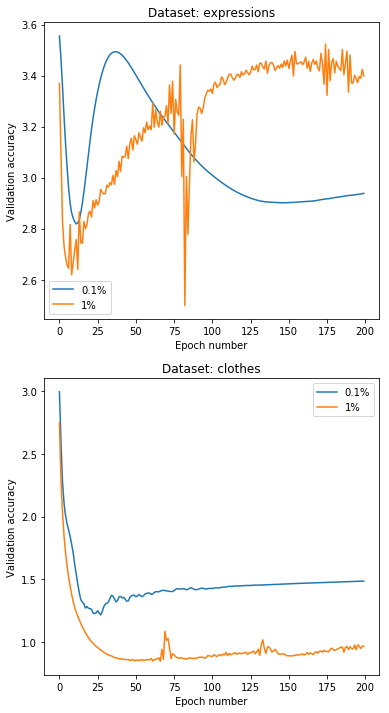
\includegraphics[scale=0.5]{behaviour.png}
            \caption{Comparison of the evolution of the validation error when the sizes of the datasets are 1\% and 0.1\%. The effects of over-fitting are clearly more dramatic for expressions that for clothes. The system presents a better behaviours when classifying clothes. }
            \label{fig:tf_beh}
        \end{center}
    \vskip -5mm
\end{figure*}

\subsubsection{\textbf{Interpretation and Discussion}}

The proposed system provided some benefits when the number of samples in the datasets is small. Depending on the context of analysis, these benefits can be higher for one dataset or the other. At first, transfer learning seems to be more effective for the clothes dataset than for the expressions dataset as seen in Figure \ref{fig:tf_clot} and Figure \ref{fig:tf_exp}. This information can give some clues about the complexity of the images in every dataset. At a glance, the experimental results allows to say that the features extracted from the clothes are less challenging to learn than those extracted from the expressions.

A further analysis makes possible to say that the knowledge obtained by VGG16 from the ImageNet dataset was more beneficial for the expressions dataset in terms of relative gain. The validation accuracy ratios between the transfer learning and the baseline experiments are 1.5 and 1.56 for the clothes and expressions dataset respectively. This might indicate that VGG16 extracted features that were more relevant for expressions than for clothes.

In absolute values, the knowledge from VGG16 in terms of validation accuracy was more beneficial for the clothes dataset. The additional validation accuracies obtained from transfer learning compared to the baseline system were 0.25 and 0.18 for the clothes and expressions dataset, respectively, as seen in \ref{tab:tf_3}. Even though the extracted features from VGG16 could have been more relevant for expressions, they were good enough to increase the performance of the system for clothes.

However, the additional validation accuracies compared to the data augmentation experiments are -0.01 and 0.06. Therefore, the benefits of data augmentation are comparable to the benefits of transfer learning for the clothes dataset. One possible explanation is in the kind of information obtained from images. 

Convolutional layers extract information about the local spatial correlation of images. The result of this process is the detection of edges, shapes, patterns and other geometric information. The baseline system was shallow and only contained one convolutional layer. Thus, the geometric information extracted from this single layer along with data augmentation provided enough elements to increase the performance in the classification task in a way that it was comparable to the benefits obtained from transfer learning. 

When comparing the benefits of transfer learning under the conditions of low and high number of samples, the results are dis-pair. First, the benefits are higher when the number of clothes samples is higher as seen in \ref{tab:tf_3}. The relative and absolute gains are higher when using 100\% of the clothes dataset. In the other hands, the benefits are higher when the number of expressions samples is lower. The relative and absolute gains are higher when using only 1\% of the expressions dataset.

\subsection{Siamese Neural Network}

\subsubsection{\textbf{Motivation}}

[[PLACEHOLDER]]

\subsubsection{\textbf{Description}}

[[PLACEHOLDER]]

\subsubsection{\textbf{Results}}

[[PLACEHOLDER]]

\subsubsection{\textbf{Interpretation and Discussion}}

[[PLACEHOLDER]]

\section{Related Work}

One of the motivations for transfer learning was taking advantage of previous work. One of the benefits of this approach is the saving of computational resources. The available pre-trained networks for computer vision tasks were developed by feeding them with several million of images and using a considerable number of computational resources. Both components, big amounts of data and a high number of computational resources, are not available for every organization or people. Therefore, transfer learning provides a way to obtain the benefits of neural networks under those circumstances.

Previous work that took advantage of transfer learning in the context of small data includes \citep{ng2015deep}. This project tried to adapt the knowledge from a convolutional neural network trained on ImageNet to a classification task related to the recognition of facial expressions using two new datasets. The approach implemented by the authors included a cascade fine-tuning methodology where the pre-trained network was first adapted to one dataset, then a further adaptation was performed using the second dataset. The best validation accuracy in their experiments was 0.49, close to 0.50 presented in this report. This result could confirm the level of complexity to classify facial expressions.

Other experiments on small dataset have made comparisons between shallow and deep architectures to minimize the effects of overfitting \citep{pasupa2016comparison}. The results of these experiments statistically demonstrated that shallow models did perform better than deep ones with no regularization. However, a combination of various regularization techniques increased the performance of the deep models. As described in the configuration of the simple transfer learning in this report, the use of regularization techniques did provide some robustness to cope with overfitting as seen in Figure \ref{fig:tf_beh}.

Further work can be aimed to investigate the effects of transfer learning in combination with data augmentation for small data. As seen in Table \ref{tab:tf_2}, the accuracy gain of transfer learning and data augmentation are comparable, especially for clothes. A combination of both approaches could potentially increase the performance of the model more than using them independently.

\section{Conclusions}
\label{sec:conclusions}

As per the results of the experiments presented previously, there are two main conclusions in regards to transfer learning and small data. First, it is clearly evident that the use of transfer learning improved the performance of the classification task under conditions of small data for both datasets, which proves the first of the hypotheses.

The increase of the performance in terms of validation accuracy not only depends on the simple use of transfer learning. Hyper-parameters like the learning rate are still critical in the behaviour of the system. Moreover, an improper value for such hyper-parameter can not even make any improvement compared to random choice. 

Another thing to note is the lose of flexibility in the management of the images. The raw images provide information about the pixel intensity. This type information can be processed in several ways. One of the options is to perform affine transformations, a technique that was previously utilised to implement data augmentation.

However, once the images were passed through the convolutional layers of VGG16, the pixel intensity information was transformed to another representation space. This new representation of the information might not be as easy to understand as pixel intensities. It is known that this information represents the local spatial correlation of the images. However, modifying it in a similar way raw images are modified might not provide similar results.

Since, the transfer learning technique was also utilised for bigger sizes of the dataset, it was possible to compare the effects of this technique when more data is available. It was clear, that the benefits of transfer learning were more evident for small data when using the expressions dataset, which partially proves the second hypothesis. However, this does not mean that transfer learning can be discarded when the amount of data is sufficiently big. It is worth to remember that transfer learning is also a way to work when the computational resources are limited.

The benefits of transfer learning in terms of the target dataset depends on the context of analysis. As discussed previously, in relative values, the use of transfer learning was more beneficial for the expressions dataset. However, the absolute increment of the validation accuracy was higher for the clothes dataset. This analysis gives more insight about the relationship between the datasets used to pre-train a network and the datasets used during transfer learning. 

Evidently, the benefits of transfer learning depend on the characteristics of the target dataset. It follows that some expertise is needed in order to understand the differences and similarities of the source dataset (used to pretrain the network) and the target dataset (used to apply transfer learning). This way the benefits of transfer learning can be maximized while the risks are minimized.

[[PLACEHOLDER ONE SHOT]]


\bibliographystyle{abbrv}
\bibliography{example-refs}

\end{document}
